\documentclass[handout, navsym]{tum-presentation}

\graphicspath{{figs/}}
\usepackage{fancybox}
\usepackage{listings}
\usepackage{xcolor}

\setbeamercovered{invisible}
\setbeamertemplate{navigation symbols}{}
\setbeamertemplate{section in toc}[sections numbered]
\setbeamertemplate{subsection in toc}[subsections numbered]
\setbeamertemplate{subsubsection in toc}[subsubsections numbered]
\numberwithin{equation}{section}

\definecolor{dkgreen}{rgb}{0,0.6,0}
\definecolor{gray}{rgb}{0.5,0.5,0.5}
\definecolor{mauve}{rgb}{0.58,0,0.82}

\lstset{
	basicstyle=\footnotesize\ttfamily,% 基本风格
         numbers=left,    % 行号
         numberstyle=\tiny,
         numbersep=10pt,  % 行号间隔 
         tabsize=2,       % 缩进
         extendedchars=true, % 扩展符号?
         breaklines=true, % 自动换行
         language=C++,
         frame=shadowbox,  % 框架左边竖线
         xleftmargin=19pt,% 竖线左边间距
         showspaces=false,% 空格字符加下划线
         showstringspaces=false,% 字符串中的空格加下划线
         showtabs=false,  % 字符串中的tab加下划线
       xleftmargin=2em,xrightmargin=2em,aboveskip=1em
}

\title{Praktikum: Grundlagen der Programmierung}
\author[Wenjie Hou]{Wenjie Hou}
\date{2. Tutorübung}
\institute{\theuniversity\par Fakultät für Informatik}
\footline{\insertshortauthor~|~\insertshorttitle~|~2. Tutorübung}

\begin{document}

\begin{frame}[noframenumbering]
  \titlepage
\end{frame}

\begin{frame}[t]
  \frametitle{Overview}
 \tableofcontents[section=show,subsectionstyle=show]
\end{frame}


\section{Lecture Review}

\begin{frame}
  \frametitle{Lecture Review}

  \begin{alertblock}{Control Statements in Java}
   \begin{enumerate}
  \item Decision Making
  	\begin{itemize}
	\item if...then
	\item if...then...else
	\item if...then...else if...then...
	\item Switch
	\item Ternary operation A ? B : C
	\end{itemize}
  \item Looping Statements
  	\begin{itemize}
	\item While Loop
	\item Do-While Loop
	\item For Loop
	\item Foreach Loop
	\end{itemize}
  \item Branching Statements
  \begin{itemize}
	\item Break
	\item Countinue
	\item Return
	\end{itemize}
  \end{enumerate}
  \end{alertblock}
\end{frame}

\section{P01: Summieren}
\begin{frame}[fragile]
  \frametitle{P01: Summieren}
  \vspace*{\fill}
\large  In this task, a program is to be created which calculates the sum of several integers entered by the user. Ask the user to enter a number with "$\color{blue} Bitte$ $\color{blue}Zahl$ $\color{blue} eingeben:$" \textbf{until 0 is entered}. \par
~\\
As soon as the number 0 is entered, print "$\color{blue} Summe:$", print the sum of the numbers entered by the user in another line  and \textbf{terminated} the program.\par
\bigskip
\textbf{\large Example Output:}
\center
\begin{lstlisting}
<Bitte Zahl eingeben:
>-3
<Bitte Zahl eingeben:
>31
<Bitte Zahl eingeben:
>0
<Summe:
<28
\end{lstlisting}

\vspace*{\fill}
\end{frame}


\subsection{Flow Diagram}
\begin{frame}{Flow Diagram}
\begin{figure}[htbp]
\centering
\begin{minipage}[t]{0.48\textwidth}
\centering
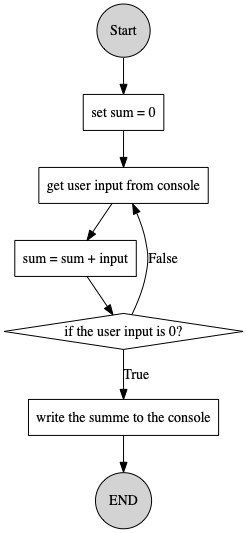
\includegraphics[height=8cm]{p1-1.png}
\caption{v1}
\end{minipage}
\begin{minipage}[t]{0.48\textwidth}
\centering
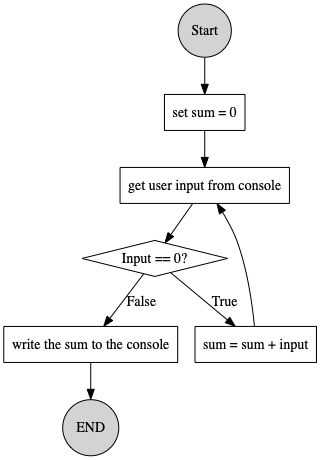
\includegraphics[height=8cm]{p1-2.png}
\caption{v2}
\end{minipage}
\end{figure}
\end{frame}

\subsection{Code - 1}
\begin{frame}{Code -1}
\center 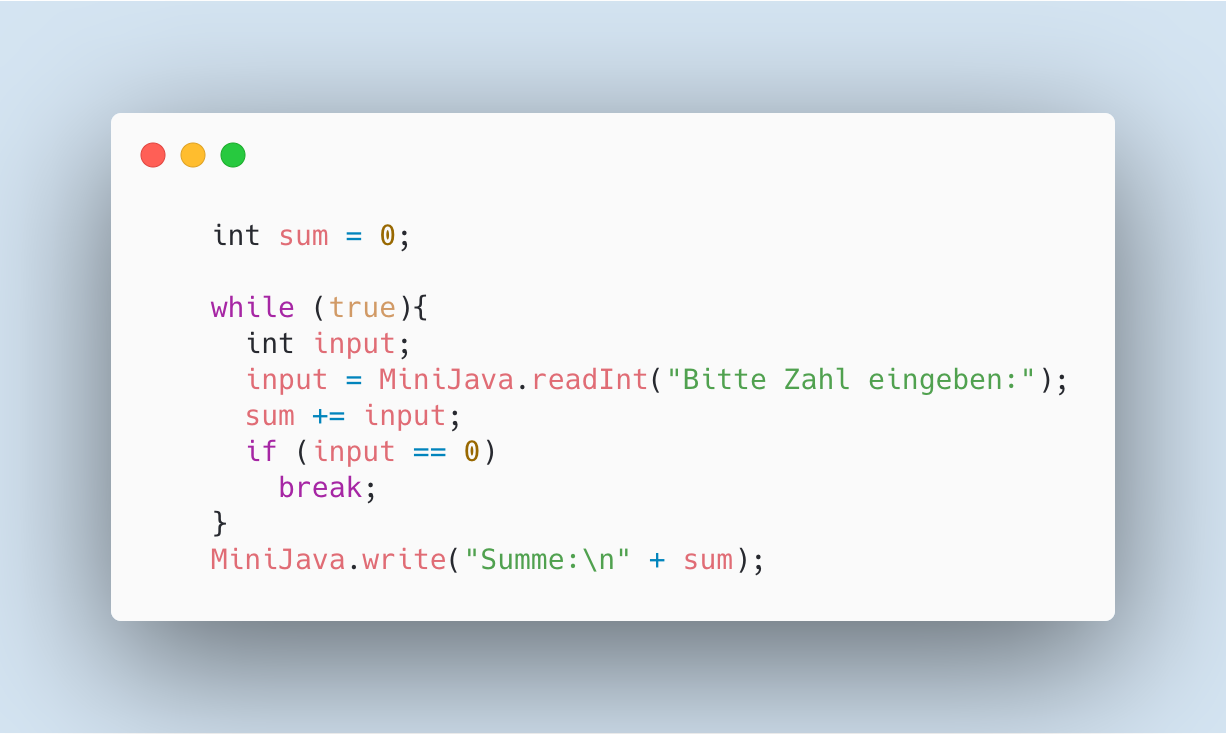
\includegraphics[height=9cm]{p1-code.png}
\end{frame}

\subsection{Code - 2}
\begin{frame}{Code -2}
\center 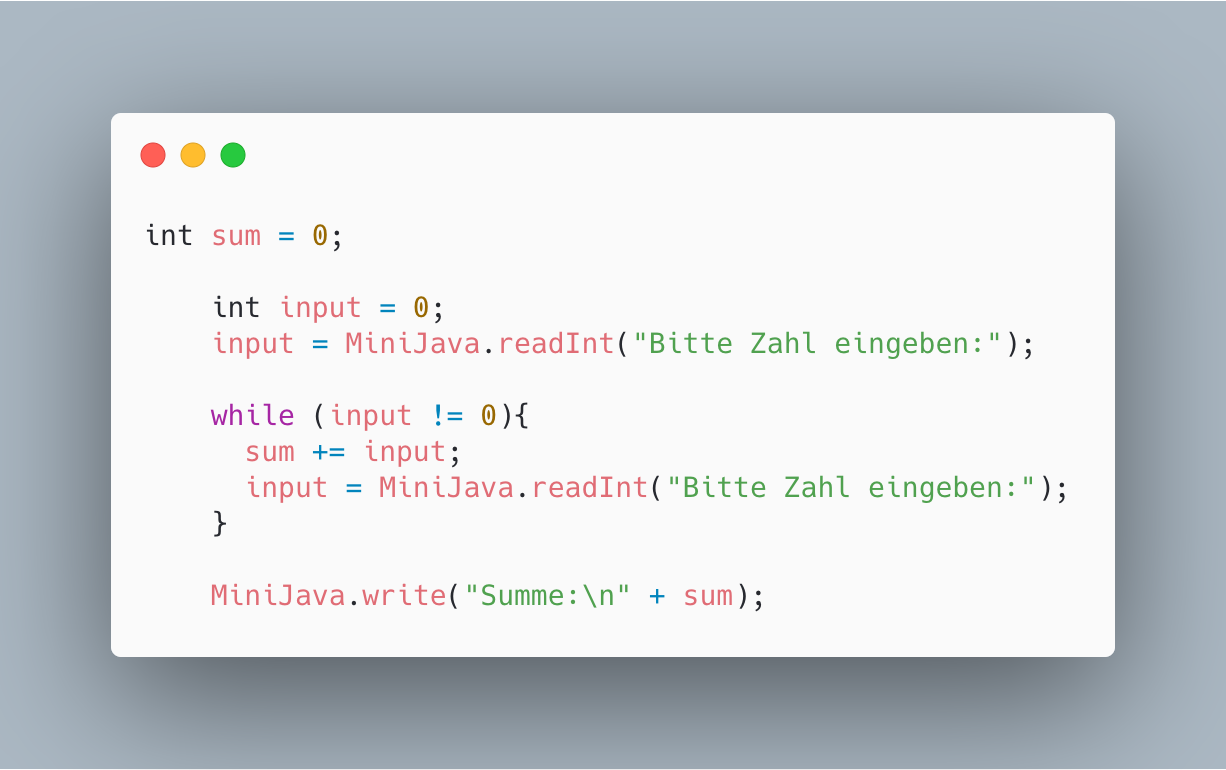
\includegraphics[height=9cm]{p1-2-code.png}
\end{frame}

\section{P02: Integer factorization}
\begin{frame}[fragile]
\frametitle{P02: Integer factorization}
\vspace*{\fill} \large
Any natural number $n > 1$ is either a prime itself or can be represented as a product of prime numbers. To calculate the prime factorization of a number $n$, divide it by all natural numbers starting from 2. If a divisor t is found, then output t. If the quotient $\frac{n}{t} > 1$, then it is also decomposed into its prime factors.\par
~\\
Write a MiniJava program that says\textsl{ \color{blue}"Bitte Zahl eingeben:"} and reads a natural number $n > 1$ from the user and breaks it up into prime terms. Your program should output all prime factors of the number $n$ separated by spaces on the screen. If the input number entered is $n \leq 1$, then print \textsl{\color{blue}"Fehler: $n >1$ erwartet!"}.\par
~\\
Tip: You can use the $\color{blue}writeConsole ()$ method to print something on the console without extra line break. By using method $\color{blue}writeLineConsole()$ you can print a line with the line feed.\par
\bigskip
\textbf{\large Example Output:}
\begin{lstlisting}
Bitte Zahl eingeben:
>12321342
2 3 3 3 11 20743
\end{lstlisting}
\vspace*{\fill}

\end{frame}

\subsection{Flow Diagram}
\begin{frame}[fragile]
\frametitle{Flow Diagram}

\center 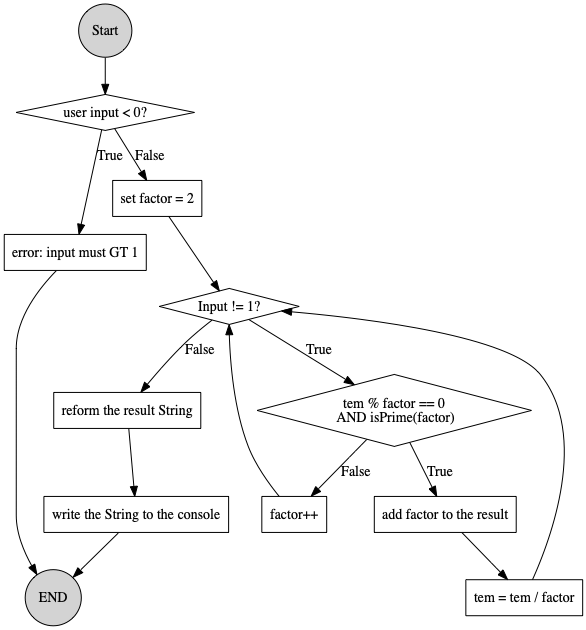
\includegraphics[height=9cm]{p2.png}

\end{frame}

\subsection{Code}
\begin{frame}[fragile]
\frametitle{Code}

\center 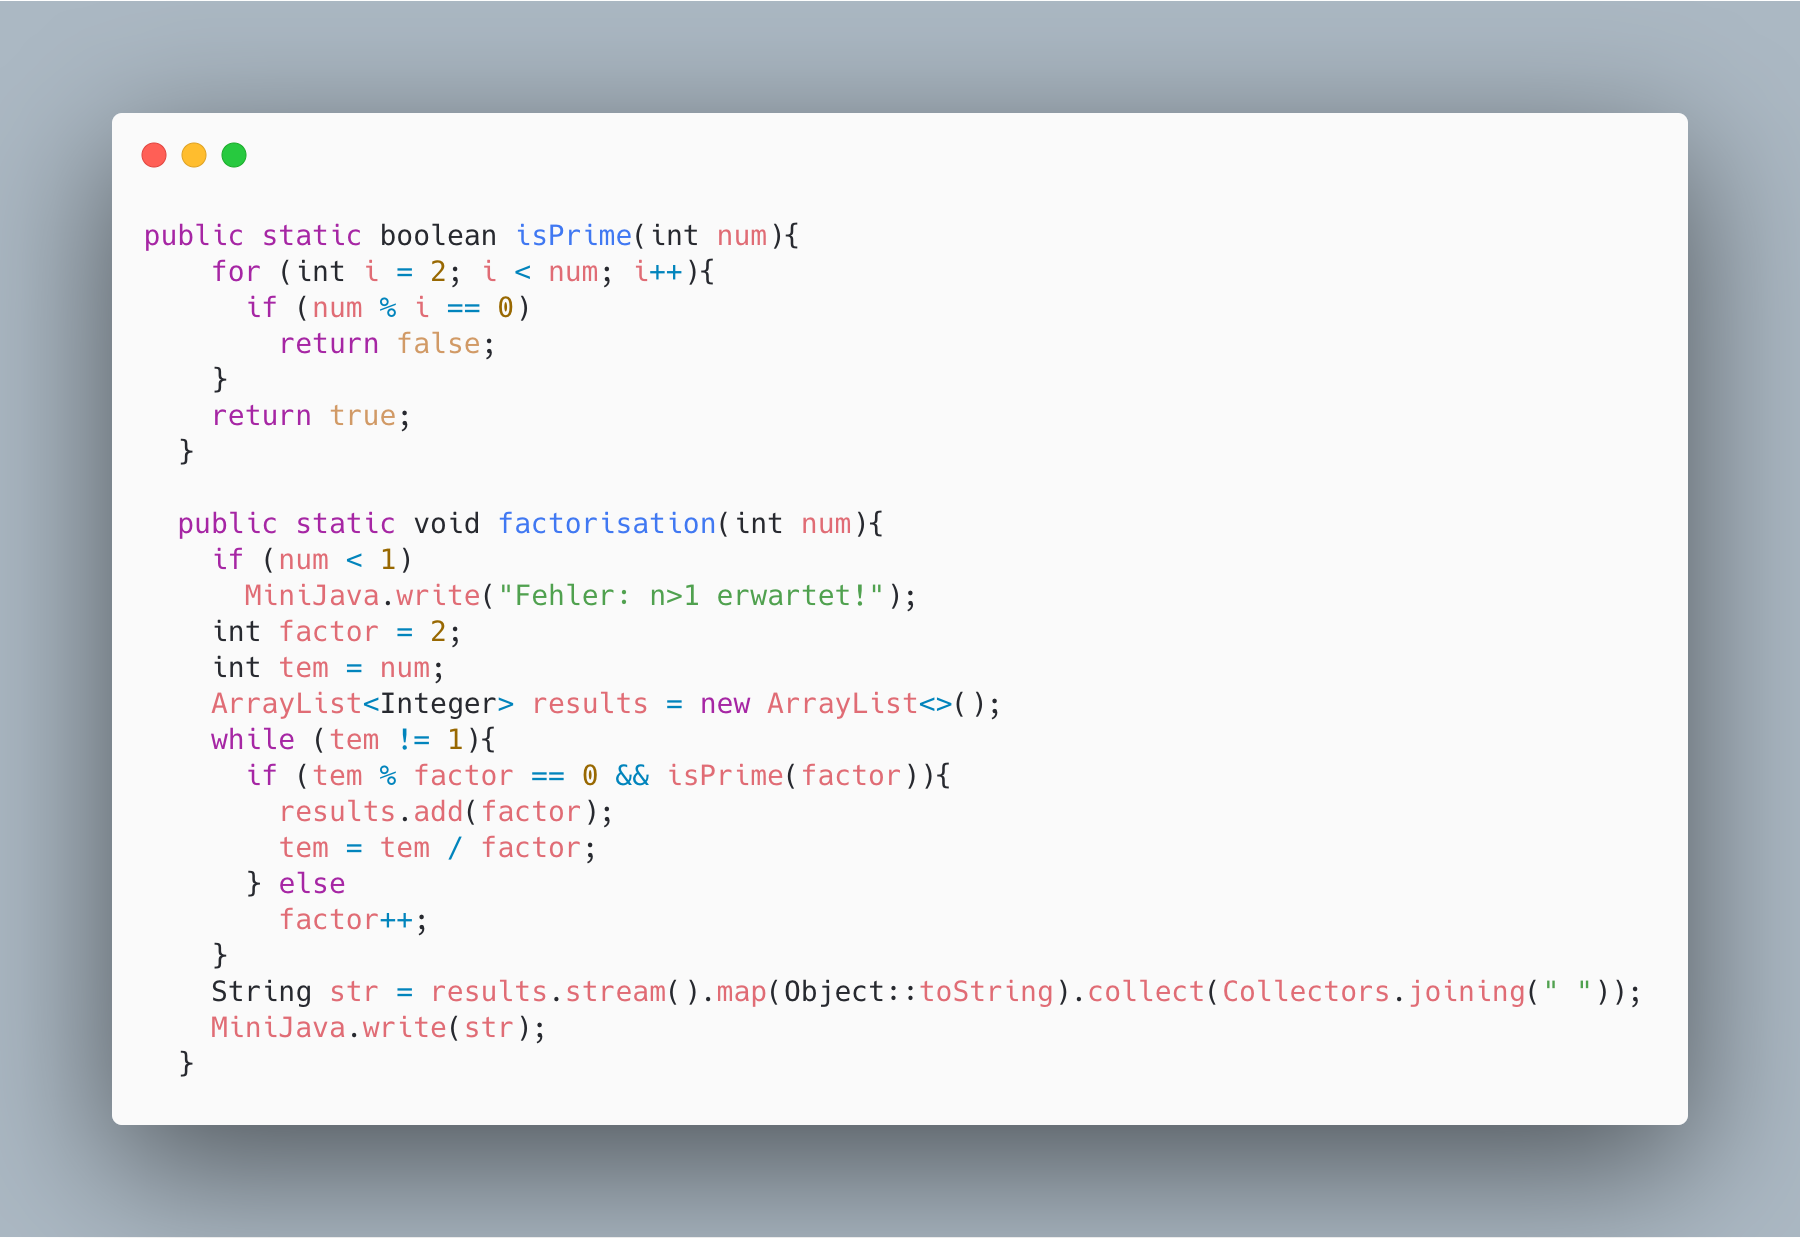
\includegraphics[height=9cm]{p2-code.png}

\end{frame}

\section{P03: Population of Rabbit}
\begin{frame}[fragile]
\frametitle{P03: Population of Rabbit}
\vspace*{\fill} \large

We put a pair of mature rabbits on a desert island to find out how many rabbits will born within a year. It is assumed that every mature couple will give birth to a new pair of rabbits each month. Each rabbit pair is sexually mature for the first month of life and each rabbit has \textbf{a lifetime of $3$ months}.\par
~\\
Write a MiniJava program that reads in the number $n$, which is the $n^{th}$ month. Your program should print out the sum of the rabbit pairs, which are mature in the $n^{th}$ month. You can assume that $n \geq 1$. \par
\bigskip
\textbf{\large Example Output:}
\begin{lstlisting}
<Bitte Zahl eingeben:
>3
<4
\end{lstlisting}
\vspace*{\fill}
\end{frame}

\subsection{Code}
\begin{frame}[fragile]
\frametitle{Code}

\vspace{-2cm}
\center 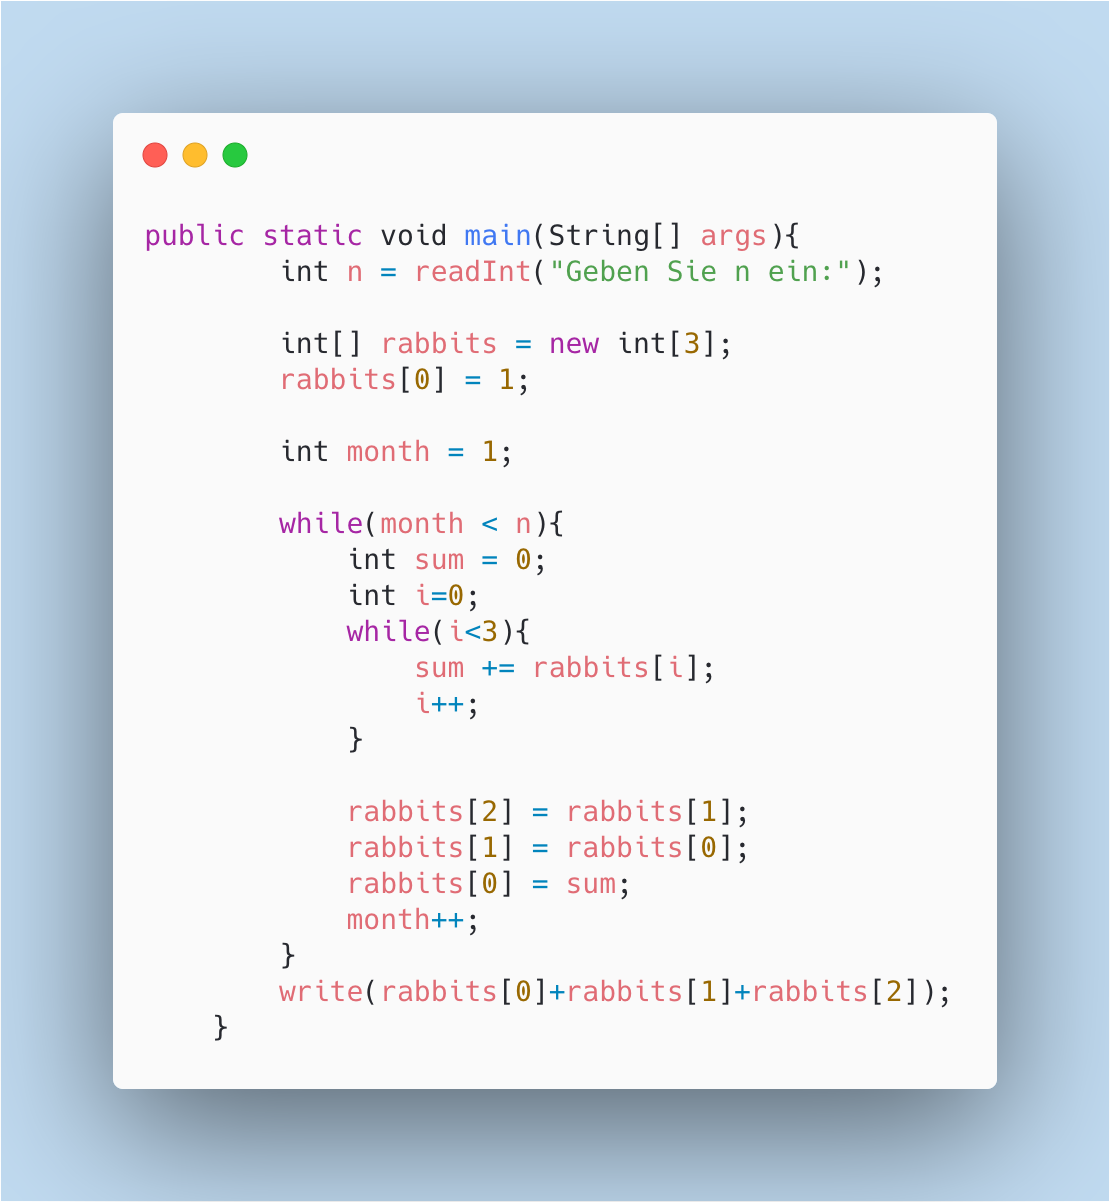
\includegraphics[height=11cm]{p3-code.png}

\end{frame}

\section{P04: 3 and 7}
\begin{frame}[fragile]
\frametitle{P04: 3 and 7}
\vspace*{\fill} \large

Write a program that prints \textsl{ \color{blue}"Bitte Zahl eingeben:"}" and then read in a number $n$. Then it calculate the sum of all positive numbers less than or equal to n, and are divisible by 3 or 7. Then print the result to console. If the user enters a negative number,\textsl{\color{blue}"Fehler: $n >1$ erwartet!"} and exit the program.\par
~\\
If the user types e.g. If the number is $25$, so we add $3, 6, 7, 9, 12, 14, 15, 18, 21, and 24$ and it gives us $129$.\par
\bigskip
\textbf{\large Example Output:}
\begin{lstlisting}
Bitte Zahl eingeben:
>91
1822

Bitte Zahl eingeben:
>16
1822
\end{lstlisting}

\vspace*{\fill}
\end{frame}

\subsection{Code}
\begin{frame}[fragile]
\frametitle{Code}

\center 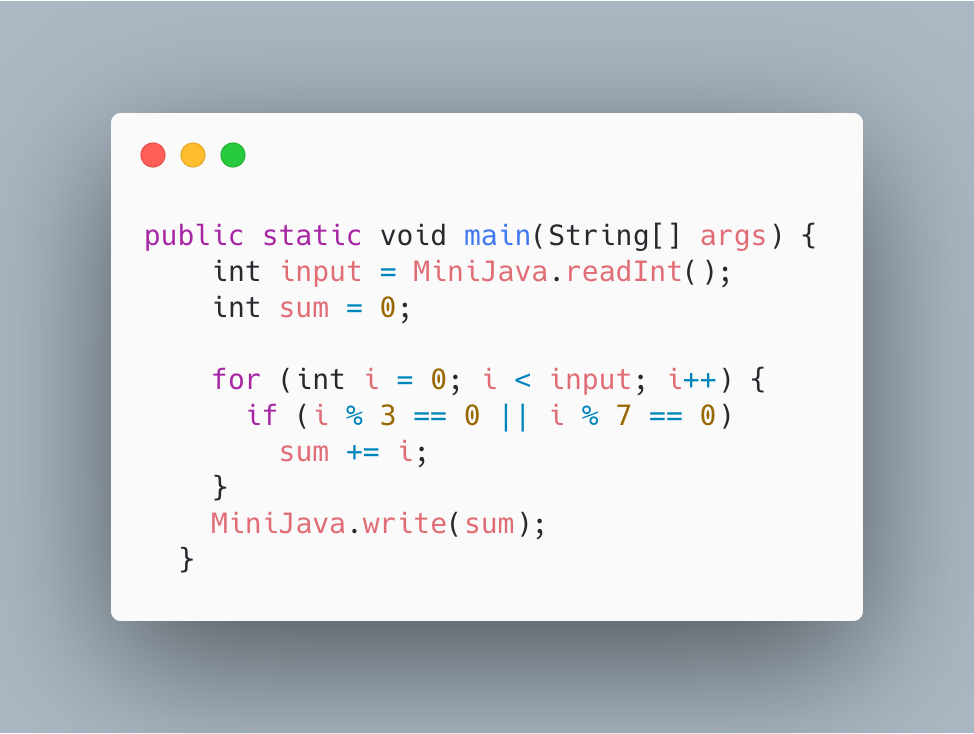
\includegraphics[height=9cm]{p4-code.png}

\end{frame}

\begin{frame}[fragile]
\vspace*{\fill} 
\begin{center}
 \Huge Thank You!
\end{center}
\vspace*{\fill} 
\end{frame}




\end{document}
